% Lab Writeup for HD Lab
% Adam Reyes, George Wong
% Advanced Lab Fall 2013


\documentclass[paper=a4, fontsize=11pt]{scrartcl} % A4 paper and 11pt font size
\usepackage[left=2.5cm,top=2.5cm,right=2.5cm,bottom=2.5cm]{geometry} 
\usepackage{amsmath}
\usepackage{graphicx}
\usepackage{sectsty}
\usepackage{fancyhdr}
\pagestyle{fancyplain}
\usepackage{subcaption}
\usepackage{wrapfig}
\usepackage[english]{babel}
\usepackage{float}

\numberwithin{equation}{section}
\numberwithin{figure}{section} 
\numberwithin{table}{section}
%\setlength\parindent{0pt}

\fancyhead[R]{\thepage} 
\fancyhead[L]{Reyes, Wong} 
\fancyhead[C]{Hydrogen-Deuterium Shift} 
\fancyfoot[L]{} 
\fancyfoot[C]{} 
\fancyfoot[R]{} 

\newcommand{\horrule}[1]{\rule{\linewidth}{#1}}

\title{	
The Hydrogen-Deuterium Isotope Shift
\horrule{0.5pt}
\normalfont \normalsize 
\textsc{Advanced Experimental Physics }
}

\author{Adam Reyes \\ George Wong} % Your name

\date{\normalsize\today} % Today's date or a custom date


\begin{document}
\maketitle



%%%%%%%%%Abstract%%%%%%%%%%%%%%%%%%%%%
\textbf{Abstract:}
Through use of a grating spectrometer, the spectra of both hydrogen and deuterium are measured. Through calculations, the difference in the spectra can be related to the mass difference between a single proton and a proton-neutron pair.

%%%%% INTRODUCTION %%%%%
\section{Introduction}

\subsection{Theory}

The Bohr model of the Hydrogen Atom gives that the allowed energies of
the atom's electron are
\begin{equation}
\label{eq:Hen}
E_n = -\frac{R_E}{n^2}
\end{equation}
Where $R_E$ is the Rydberg energy and $R_E \propto \mu$. Here
$\upsilon$ is the reduced mass of the nucleus and the electron. If we
consider now the isotope of Hydrogen, deuterium, with one neutron it
clearly has a different $\mu$ from plain Hydrogen. So the energy of
the allowed transitions and hence the emission spectrums are
different. The Rydberg formula(eqn \ref{eq:emis}) gives the wavelengths of the emission
spectrum for Hydrogen with an infinitely massive nucleus in terms of
the Rydberg constant $R$.
\begin{equation}
\label{eq:emis}
\frac{1}{\lambda_\infty} = R(\frac{1}{n_1 ^2}-\frac{1}{n_2 ^2})
\end{equation}
Eqn \ref{eq:lamM} gives the the emitted wavelength corrected for the
mass of the nucleus $M$.
\begin{equation}\label{eq:lamM}
\lambda_M = \lambda_{\infty} (1 + \frac{m_e}{M})
\end{equation}
where $m_e$ is the mass of the electron. From this it can be shown
that the mass shift from Hydrogen($M_H$) to Deuterium($M_D$) is
\begin{equation}
\Delta M = \frac{\Delta \lambda}{\lambda_\infty}\frac{M_D M_H}{m_e}
\end{equation}
difference in reduced masses causes a difference in spectra between hydrogen and deuterium ``isotope shift''



* talk about best angle of incidence *

* talk about the orientation of the grating (upside down vs. right side up) *

\subsection{Setup/Apparatus}

A diffraction grating is a reflective material that has had grooves etched into its surface. Incident light reflects off of the surface and, due to interference effects, is refracted by different amounts. Equation~\ref{eq:gratingEqn} gives the relations between incident angle $\alpha$, reflected angle $\beta$, wavelength $\lambda$, and grating resolution $d$.

\begin{equation} \label{eq:gratingEqn}
n \lambda = d ( \sin(\alpha) + \sin(\beta))
\end{equation}

Figure~\ref{fig:diagram1} provides an overhead view of the apparatus.


\begin{figure}[H] \begin{center}
  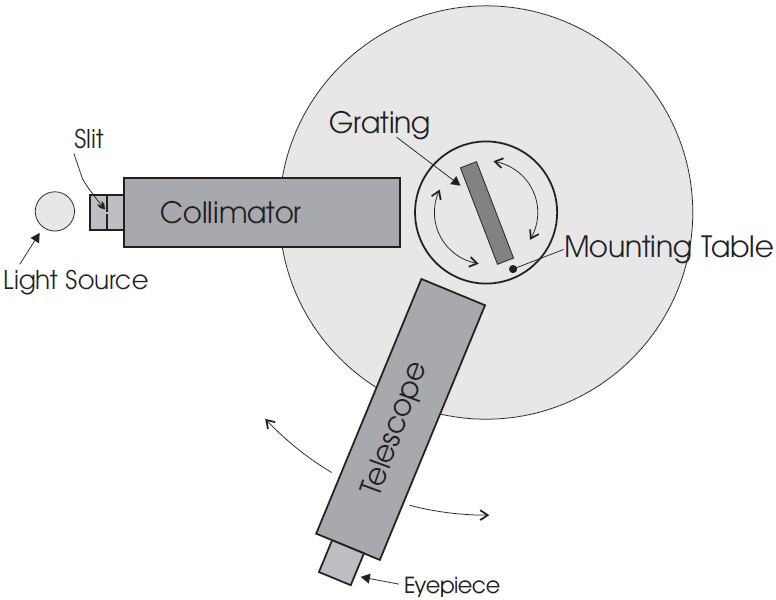
\includegraphics[height=60mm]{diagram1.png}
  \caption{\textbf{Overview of Apparatus} showing relative locations of light source (lamp), collimator with slit, diffraction grating mounted on revolving table, telescope (also on revolving table) and eyepiece.}
  \label{fig:diagram1}
\end{center} \end{figure}



%%%%% PROCEDURE %%%%%
\section{Procedure}

\subsection{Calibration}

It was important to ensure all parts of the apparatus were focused and adjusted so that the light coming from the slit would diffract off of the grating and enter the telescope at proper angles for viewing.

\begin{enumerate}
\item A two-sided mirror was placed on the mounting table and centered. Its exact location was marked for repeatability.
\item The telescope was then focused to the image of the crosshairs in
  the eyepiece reflected from the mirror.
\item The telescope and mounting table were leveled to each other by
  aligning the horizontal crosshair of the eyepiece to the reflected
  image on both sides of the mirror using the leveling screws of the
  mount and the telescope.
\item The mirror was removed from the central mounting table and the telescope and collimator were brought to be in line with each other.
\item A light was placed behind the slit on the collimator and the distance of the lens in from the slit within the collimator was adjusted until the image of the slit as seen through the eyepiece was as focused as possible.
\item The cross hairs were positioned immediately on the slit and half way up the slit, so as to align the plane of the collimator with that of the telescope/mounting table (already aligned).
\end{enumerate}


\subsection{Angular Alignment}
\label{sec:angal}
Knowledge of the exact measures of angles was very important in this
lab, so the following method was developed to permit precise
measurements of angles. The following assumes the experimenter wishes
to generate a set up with incident angle $\alpha$, between the
collimator and normal incidence to the grating.

\begin{enumerate}
\item The telescope was aligned to normal incidence with the mirror by
  aligning the vertical crosshair of the eyepiece with its reflected image. 
\item With the position of the mount fixed, the telescope was rotated
  by the desired angle $\alpha$.
\item The relative angle of the telescope and mounting table was
  fixed, and the two pieces were moved together until the reflection
  from the slit image was aligned with the vertical crosshair. 
\item At this point, the incident and reflected angles were equal and exactly $\alpha$. The angular position of the mounting table was fixed.
\end{enumerate}

\subsection{Eyepiece Calibration}
\label{sec:eyecal}

In order to make precise angular measurements for this experiment we
used an eyepiece with a thing crosshair that could be moved with a
micrometer screw gauge. The divisions on the gauge had to be
calibrated in order to know what grating angle is swept through as the
screw is turned. This was done by picking two lines separated by as
much arc length as could fit in the view of the eyepiece. This angle
was then measured using the protractor on the spectrometer, then
measured using the eyepiece gauge. It was then determined that one
eyepiece unit corresponds to $0.0023\pm0.0001^{\circ}$
\subsection{Measurement of Spectra}
\label{sec:specmes}
In this section, we actually measure the spectra of the light (emission spectra) as a function of angle. The following procedure was performed with both the provided Sodium and Hydrogen-Deuterium lamps; however, it would be exactly the same for any lamp/source.

\begin{enumerate}
\item An angle of incidence $\alpha$ was obtained using the procedure
  outlined in~\ref{sec:angal}.
\item A light source (lamp) was placed before the slit and was covered with a blackout sheet, so as to completely darken the room.
\item The telescope was rotated from the zeroth order reflection until a line was visible. At this point, the cross hairs were brought to rest directly on the center of the line. The relative change in angle off zeroth order is noted.
\item The above step was repeated until the telescope could not be physically rotated any further.
\end{enumerate}




%%%%% DATA + ANALYSIS/RESULTS %%%%%
\section{Data \& Analysis}




%\begin{table}[H]
%\centering
%\caption{Average frequency difference ($\Delta$GHz) between peaks with associated error}
%\begin{tabular}{ || c | c c c c || }
%  \hline
%  \hline
%   $-$ & 87a & 85a & 85b & 87b \\
%  \hline
%  87a & $-$ & $2.37 \pm 0.14$ & $4.97 \pm 0.23$ & $6.03 \pm 0.53$ \\
%  85a & $2.37 \pm 0.14$ & $-$ & $2.60 \pm 0.13$ & $3.64 \pm 0.18$ \\
%  85b & $4.97 \pm 0.23$ & $2.60 \pm 0.13$ & $-$ &  $1.04 \pm 0.07$ \\
%  87b & $6.03 \pm 0.53$ & $3.64 \pm 0.18$ & $1.04 \pm 0.07$ & $-$  \\
%  \hline
%  \hline
%\end{tabular}
%\label{table:freqOffset}
%\end{table}


\section{Conclusion}


Over the course of performing the experiment, it was found that many of the procedures were difficult or impossible to perform well due to the condition of the apparatus (especially grating). In future experiments, a less-worn grating with perhaps a finer resolution would be very useful. Also, a better way to measure angles would be useful.

** talk about focusing in on a single line **


%%%%%%%%%%%%%References%%%%%%%%%%%%%%%%%%%%
%\begin{thebibliography}{99}
%\bibitem{vanier}Jacques Vanier. Relaxation in rubidium-87 and the
%  rubidium maser. Phys. Rev., 168:129-149, 1968.
%\bibitem{harvard}"Rubidium Fluoresence." Cfa.harvard.edu. Harvard, n.d. Web.
%\end{thebibliography}


% %%%%%%%%%%%%%% Absorption figure%%%%%%%%%%%%%%%%%%
% \begin{figure}[h]
%   \centering
%   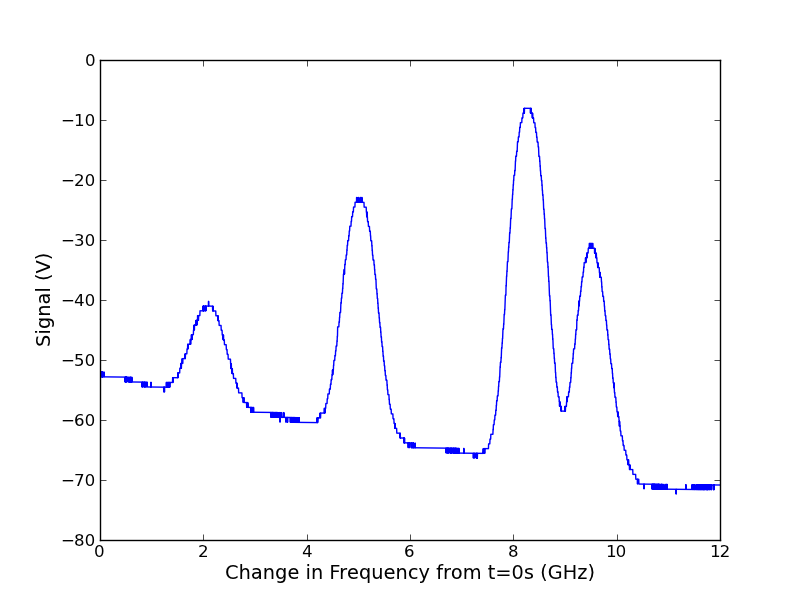
\includegraphics[width=3in]{/Users/adamreyes/Dropbox/AdvancedLab/Diode-Laser-Spec/WriteUp/figures_laserspec/ag-4-2-001_freq.png}
%   \caption{Measured Transmission Absorption Spectrum for Rubidium.}
%   \label{fig:absorption}
% \end{figure}
% %%%%%%%%%% 
% %%%%%%%%%%%%%%%%%% Saturated Absorption figure%%%%%%%%
% \begin{figure*}[h]
%   \centering
%   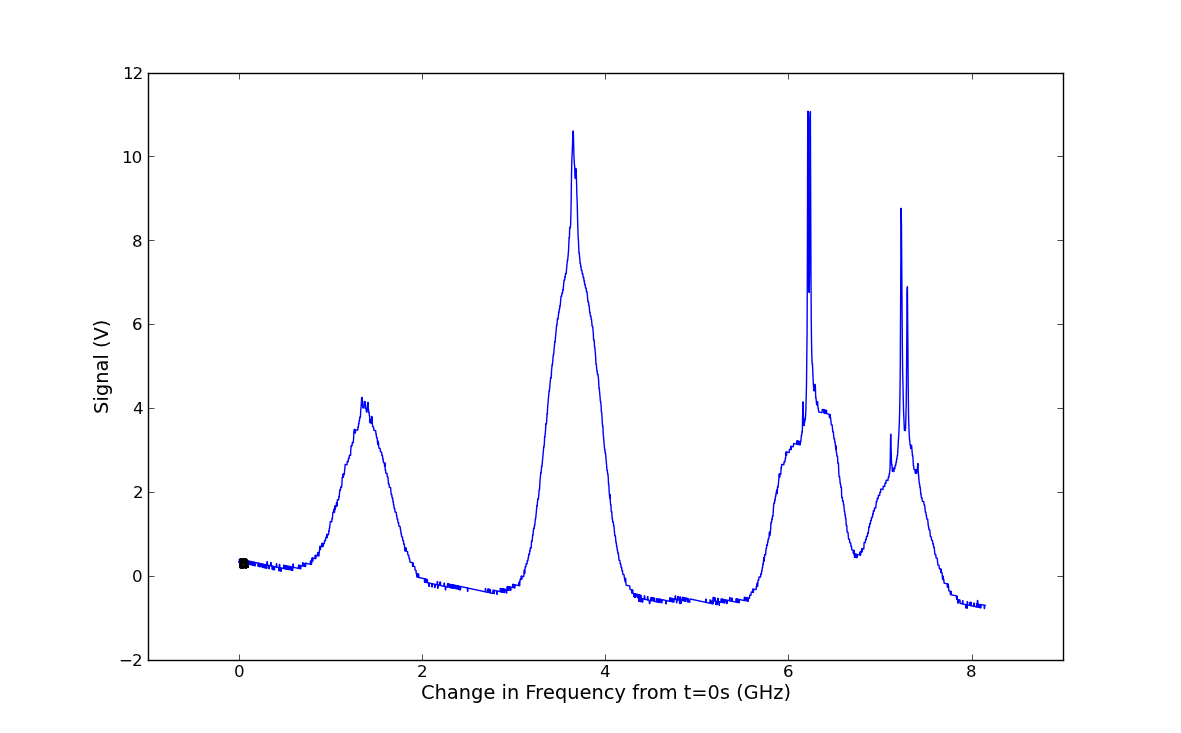
\includegraphics[width=3in]{/Users/adamreyes/Dropbox/AdvancedLab/Diode-Laser-Spec/WriteUp/figures_laserspec/ag-4-2-009_saturated.png}
%   \caption{Measured Saturated Absorption Spectrum for Rubidium with electronic subtration of doppler broadening and laser current modulation}
%   \label{fig:saturatedabsorption}
% \end{figure*}
% %%%%%%%%%% 


\end{document}